\documentclass{article} % For LaTeX2e
\usepackage{nips13submit_e,times}
\usepackage{hyperref}
\usepackage{url}
\usepackage{amsmath}
\usepackage{amssymb}
\usepackage{amsthm}
\usepackage{bm}
\usepackage{graphicx}
%\documentstyle[nips13submit_09,times,art10]{article} % For LaTeX 2.09

\title{Toxic Comment Categorization using Bidirectional LSTMs with Attention}

\author{
Michael Baumer \\
Department of Physics\\
Stanford University\\
\texttt{mbaumer@stanford.edu} \\
\And
Anthony Ho \\
Department of Applied Physics \\
Stanford University \\
\texttt{ahho@stanford.edu} \\
}

% The \author macro works with any number of authors. There are two commands
% used to separate the names and addresses of multiple authors: \And and \AND.
%
% Using \And between authors leaves it to \LaTeX{} to determine where to break
% the lines. Using \AND forces a linebreak at that point. So, if \LaTeX{}
% puts 3 of 4 authors names on the first line, and the last on the second
% line, try using \AND instead of \And before the third author name.

\newcommand{\fix}{\marginpar{FIX}}
\newcommand{\new}{\marginpar{NEW}}

\nipsfinalcopy % Uncomment for camera-ready version

\begin{document}


\maketitle

\begin{abstract}
Toxic online comments are a challenge for websites that accept user-submitted content, and human moderation is a psychologically difficult task that does not scale well. We present a framework for using deep learning to automatically identify and categorize toxic online comments into 6 overlapping sub-categories. We employ a bidirectional LSTM architecture with an attention mechanism to achieve a mean ROC AUC of .9778 on a blind test set. We use the normalized attention weights to visualize the activation of our network in response to each word within a sentence, and find qualitative agreement with human intuition. 
\end{abstract}

\section{Introduction}

Many websites that display user-submitted content must deal with toxic or abusive comments. Human moderation may carry psychological risk to the moderators \cite{atlantic}, and is difficult to implement at scale. Potential automated solutions will require not just binary classification (acceptable vs. blocked) but fine-grained comment classifications to maintain civility without interfering with normal discourse and provide explanations to users when their posts are censored. Different websites may wish to have different policies for dealing with different kinds of toxic content. For example, a website may want to allow insulting comments while still blocking threats and identity-based hate speech. 

In this project, we attempt to improve the identification and fine-grained classification of toxic online comments in a dataset provided by a Kaggle challenge \footnote{\url{https://www.kaggle.com/c/jigsaw-toxic-comment-classification-challenge}} Our dataset consists of 159,571 comments from Wikipedia talk page edits which have been labeled by human raters for the presence of toxic behavior. The 6 types of toxicity are: \texttt{toxic}, \texttt{severe\_toxic}, \texttt{obscene}, \texttt{threat}, \texttt{insult}, and \texttt{identity\_hate}. A sample of entries from the dataset is shown in Figure \ref{fig:example_comments}.

\begin{figure}[ht]
\centering
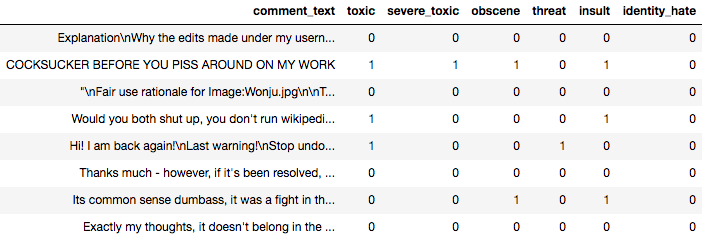
\includegraphics[width=5in]{example_comments.png}
\caption{A selection of comments from our training dataset, showing the large diversity of the corpus and the ability of a comment to have multiple labels. Also, note that while  \texttt{toxic} is a superset of \texttt{severe\_toxic}, it is not a superset of the other 4 labels.}
\label{fig:example_comments}
\end{figure}

In this report, we will describe a baseline approach to this multi-label classification task using a three-layer feed-forward neural network with averages of word-vector sentence embeddings as inputs. We will then describe our experiments with uni- and bidirectional long short-term memory (LSTM) and gated recurrent unit (GRU) architectures, and demonstrate a significant improvement in performance with the addition of an attention mechanism. Finally, we present the results of applying our framework to the dataset, including visualizations of the model's weighting of input words via the attention mechanism.

\section{Background and Related Work}

The earliest work on machine learning-based detection of online harassment can be traced back to Yin \textit{et al.} \cite{yin2009}, where they fed content, sentiment and contextual features into a support vector machine to classify instances of harassment. More recently, a paper by the group that created the dataset used in the Kaggle challenge \cite{prevwork} focused on binary identification of toxic comments (no fine-grained classification). They found success with relatively simple n-gram NLP methods, and left more complex methods (like LSTMs) as future work. 

In last year's CS224n class, a group of students looked at the same Wikipedia corpus and performed binary classification (personal attacks vs non personal attacks) using an LSTM architecture and word-level embeddings, a convolutional neural network (CNN) with word-level embeddings, and a CNN with character-level embeddings \cite{lastyear}. They found the CNN with character-level embeddings to be the most successful algorithm. 

For our project, we decided to take a different approach and investigate whether applying attention to this problem could improve the performance of word-level embeddings, inspired by Yang \textit{et al.} \cite{attention_paper}.

%%TODO Add more history of this problem. When did people start using NLP/DL techniques? What exactly did the group last year do?

%%TODO Add detail to attention section.

\section{Approach}

\subsection{Data and Preprocessing}

To convert the raw text data into usable form, we tokenize the input using the \texttt{nltk} package \cite{nltk}. Since each of the comments is of a different length, we pad or crop the token lists from each comment to a uniform length and mask the $\langle$pad$\rangle$ tokens in the RNN output layer (or attention layer, once we started using it). 

To represent each word token in the input comments, we perform word embedding using the 300-dimensional pretrained global vectors for word representation (GloVe) \cite{glove}, which was trained using aggregated global word-word co-occurrence statistics on 6 billion tokens from Wikipedia and Gigaword corpora \cite{gigaword} with a vocabulary size of 400k. 

Finally, we create input vectors of \texttt{int32} word indices using the \texttt{word2id} mappings included with the pretrained GloVe vectors. We held back a random 30\% of the training data to use as a dev set for testing the out-of-sample performance of our models.

Many offensive words posted online are not a part of the 400k words that form the GloVe vocabulary, and therefore map to the $\langle$unk$\rangle$ token. Since identifying such offensive words should improve our performance, if a token contains as a substring any member of a list of common vulgarities that are not commonly found as substrings of inoffensive words (refer to our code for details), we map the composite token to the root vulgarity.

Another observation about our dataset is the large imbalance in number of examples of each label (see Table \ref{tab:class_imb}). We deal with this problem by weighting the contributions of labels inversely to their occurrence in the training data, normalized to 1 for toxic comments (the most common label). These weights cause larger gradients to backpropagate from mistakes on the rarer labels. In this way, we learn more from each example of the more uncommon labels. 

\begin{table}[ht]
\centering
\begin{tabular}{|c|c|c|}
\hline
Category & \# of examples & \% of dataset \\ \hline
No label & 143346 & 89.8\% \\
Toxic & 15294 & 9.6\% \\
Severe Toxic & 1595 & 1.0\% \\
Obscene & 8449 & 5.3\% \\
Threat & 478 & 0.3\% \\
Insult & 7877 & 4.9\% \\
Identity Hate & 1405 & 0.9\% \\
\hline
\end{tabular}
\caption{Counts of occurences of each label category, and percentages of comments in the dataset with the given label (these do not sum to 100\% because a single comment can have multiple labels).}
\label{tab:class_imb}
\end{table}

\subsection{Baseline model}

We implemented a fully-connected feedforward neural network as our baseline model. The inputs of the model are the average of the 300d GloVe embeddings of all tokens in each comment. Note that no comment padding is necessary in this model, as the averaging procedure reduces comments of any length to a uniform size.

The neural network consists of 3 hidden layers with ReLU activation function \cite{relu}, with 30, 20, 10 hidden units in each hidden layer, respectively. Since our goal is to perform multi-label classification (i.e. the toxicity labels are not mutually exclusive), the outputs of the last hidden layer is fed into a sigmoid output layer (rather than a softmax layer, which would force the 6 class probabilities to add up to 1) with 6 units, which correspond to the predicted probabilities of each of the 6 labels. The cross entropy function is used as the loss. The neural architecture can be defined as follows:
\begin{align*}
	\bm{h}_1 &= \text{ReLu}(\bm{x} \bm{W}_1 + \bm{b}_1) \\
    \bm{h}_2 &= \text{ReLu}(\bm{h}_1  \bm{W}_2 + \bm{b}_2) \\
    \bm{h}_3 &= \text{ReLu}(\bm{h}_2  \bm{W}_3 + \bm{b}_3) \\
    \bm{\hat{y}} &= \sigma(\bm{h}_3  \bm{W}_4 + \bm{b}_4) \\
    J &= CE(\bm{y}, \bm{\hat{y}}) = - \sum_{i=1}^6 y_i \log(\hat{y}_i)
\end{align*}
where
\begin{align*}
	\bm{x} \in \mathbb{R}^{B \times 300},
    \bm{h}_1 \in \mathbb{R}^{B \times 30},
    \bm{h}_2 \in \mathbb{R}^{B \times 20}, 
    \bm{h}_3 \in \mathbb{R}^{B \times 10}, 
    \bm{\hat{y}} \in \mathbb{R}^{B \times 6},
    \bm{y} \in \mathbb{R}^{B \times 6}
\end{align*}
and $B$ is the batch size. In this baseline model and throughout this work, all bias terms are initialized to zero, while all weight matrices are initialized using Xavier initialization \cite{xavier}.

With this baseline model, we found relatively good dev set performance as measured by the ROC curves for each toxicity type (see Figure \ref{fig:roc}). The mean ROC AUC across the 6 labels on the blind test set was 0.9490, which is good performance for a baseline, but placed us $0.04$ behind the leading Kaggle entry. The similarity between the train and dev set curves shows that we were not suffering from severe overfitting.
    
\begin{figure}[h]
	\centering
    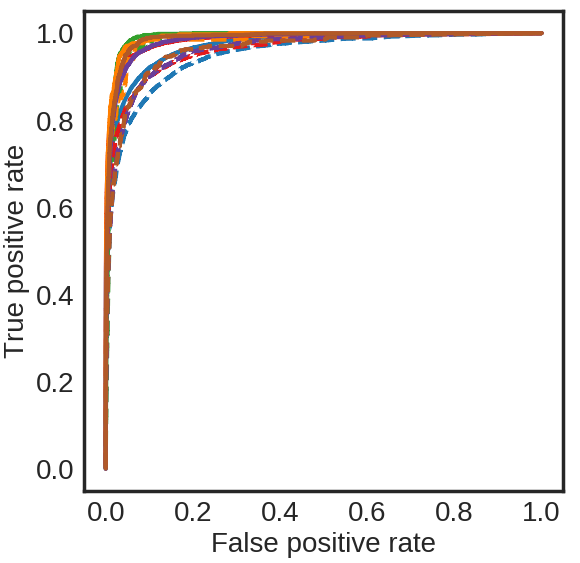
\includegraphics[height=2in]{baseline_roc.png}
    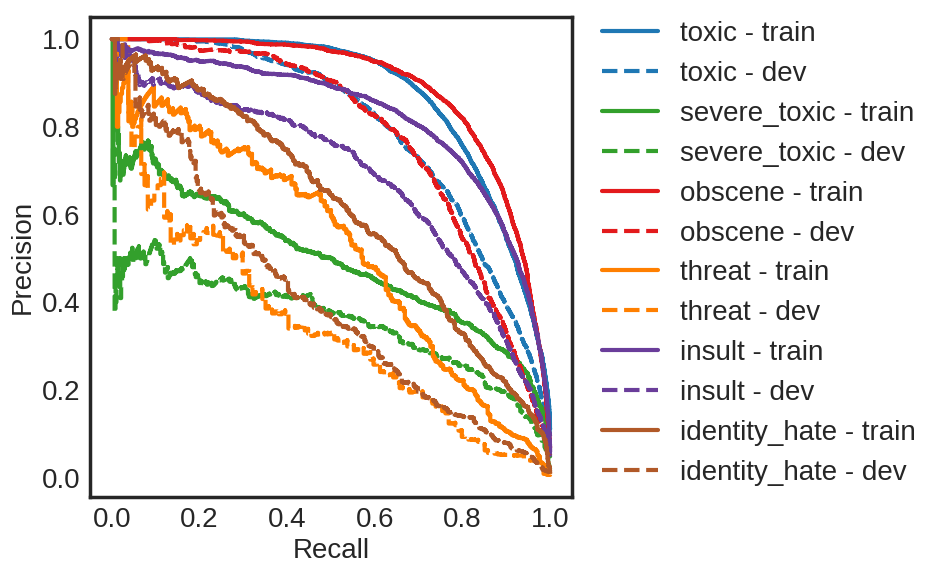
\includegraphics[height=2in]{ff_l3_h302010_f300_prc.png}
    \caption{The ROC and precision-recall curves for our baseline model's performance on each toxicity type as classified by our baseline model.}
    \label{fig:roc}
\end{figure}
   
Since the number of true negatives (non-toxic comments) in our dataset is large (see Table \ref{tab:class_imb}), and ROC curves plot the true positive rate ($TPR = TP/(TP+FN)$) vs. the false positive rate ($FPR = FP/(FP+TN)$), their appearance is biased by this imbalance in our dataset. However, since the mean AUC for these ROC curves was  the official metric of the Kaggle challenge, we used these as our primary evaulation metric. 

For a more direct measure of our classifier's performance for each label, we also plotted the precision vs. recall performance of our baseline classifier (shown at right in Figure \ref{fig:roc}). Here we see that our performance is better for the labels that have more training examples.

\subsection{Recurrent Architectures}
\label{sec:lstm}

Our baseline model achieved relatively good performance, but we thought that we could improve it by building a recurrent neural network (RNN) model that is able to use positional information of each of the words rather than an average over the entire sentence. We found that RNNs with GRU and LSTM cells were superior to a vanilla RNN architecture, but the differences between LSTM and GRU were minor, so we decided to focus on networks with LSTM cells.

We implemented our models in Python using tensorflow \cite{tensorflow}. For the LSTM cells that form the backbone of our architecture, we use the tensorflow implementation of the original LSTM equations from \cite{lstm}, shown below:
\begin{align*}
	\bm{i}_t &= \sigma \left(\bm{x}_t \bm{W}^{(i)} + \bm{h}_{t-1} \bm{U}^{(i)}\right) \\ 
    \bm{f}_t &= \sigma \left(\bm{x}_t \bm{W}^{(f)} + \bm{h}_{t-1} \bm{U}^{(f)}\right) \\ 
    \bm{o}_t &= \sigma \left(\bm{x}_t \bm{W}^{(o)} + \bm{h}_{t-1} \bm{U}^{(o)}\right) \\ 
    \bm{\tilde{c}}_t &= \tanh \left(\bm{x}_t \bm{W}^{(o)} + \bm{h}_{t-1} \bm{U}^{(o)}\right) \\ 
    \bm{c}_t &= \bm{f}_t \circ \bm{c}_{t-1} + \bm{i}_t \circ \bm{\tilde{c}}_t \\
    \bm{h}_t &= \bm{o}_t \circ \tanh (\bm{c}_t)
    \label{eqn:lstm}
\end{align*}

The LSTM architecture allows information to flow long distances across the unrolled network (if $f_t = 1$ and $i_t = 0$, the previous state flows straight through the network), but also prevent exploding gradient problems ($o_t$ modulates strength of output at each step, and $f_t = 0$ allows prior states to be forgotten so backpropagation need not continue all the way back to $t=0$). We also investigated the use of GRU cells (which have similar properties) for this task and found comparable performance to LSTM cells, so we omit their equations here \cite{gru}.

For a unidirectional LSTM architecture, it is possible to use the hidden state of the final time step as the overall output state $\bm{\tilde{h}}$ that is fed into the final output layer. We found better performance, however, when we use the element-wise average over the hidden states of all time steps (masking any hidden states at time steps where the $\langle$pad$\rangle$ token was input) as $\bm{\tilde{h}}$, the input to the final layer of our architecture.

With a bidirectional LSTM architecture, we have one set of parameters for a forward-unrolled LSTM and a separate set of parameters for a backward-unrolled LSTM that reads input token lists starting at the end rather than the beginning. For each token position, we therefore have two output states at each time step, which we either take the average of before averaging across all time steps, or concatenate to form a single joint output state which is then feed into the the attention layer described below. 

To prevent overfitting, we add regularization to the overall output state of the LSTMs (or attention layer) by applying dropout \cite{dropout} with $p_{\text{drop}} = 0.5$:
\begin{align*}
	\bm{h}_{\text{dropout}} = \text{Dropout}(\bm{\tilde{h}}, p_{\text{drop}})
\end{align*}

Finally, we use a fully-connected layer with sigmoid activations to convert the output of the dropout layer to the probabilities of each label:
\begin{align*}
	\bm{\hat{y}} = \sigma \left( \bm{h}_{\text{dropout}} \bm{U} + \bm{b} \right)
\end{align*}
where $\bm{h}_{\text{dropout}} \in \mathbb{R}^{B \times H}, \bm{U} \in \mathbb{R}^{H \times 6}$ and $\bm{\hat{y}} \in \mathbb{R}^{B \times 6}$, with $H$ as the hidden state size of the RNN/LSTM/GRU and $B$ as the minibatch size.

\subsection{Attention Mechanism}

To extract and add importance to informative words that might be relevant to the classification, we utilized a word attention mechanism as described by Yang \textit{et al.} \cite{attention_paper}. We implemented the attention mechanism by modifying publicly available code \cite{attention_code} in order to allow for masking comments with variable length. In our neural architecture, the attention mechanism can be optionally applied to reduce the set of hidden vectors $\{\bm{h}_t\}$ from every RNN/LSTM/GRU time steps $t = \{1, \dots, T\}$ to an attention output vector $\bm{\tilde{h}}$, as opposed to the averaging as described above. The attention output vector $\bm{\tilde{h}}$ is then fed as the input to the dropout layer described above. The mathematical formulation of this attention mechanism is described below:

\begin{align*}
	\bm{v}_t &= \text{tanh}(\bm{h}_t \bm{W}_a + \bm{b}_a) \\
    s_t &= \bm{v}_t \bm{u}_a^\top \\
    \alpha_t &= \frac{\exp(s_t)}{\sum^T_{t=1} \exp(s_t)} \\
    \bm{\tilde{h}} &= \sum^T_{t=1} \alpha_t \bm{h}_t
\end{align*}

In this attention mechanism, the hidden vectors of each word $\bm{h}_t$ from the recurrent time step $t$ is feed into a single tanh non-linearity to produce a new word representation $\bm{v}_t$. An attention score $s_t$ is then computed by measuring the dot product similarity between $\bm{v}_t$ and the word context vector $\bm{u}_a$. The attention weights $\alpha_t$ can then be computed by normalizing the attention score across all time steps via a softmax function. Finally, an attention output vector $\bm{\tilde{h}}$ is computed as the weighted sum of the original hidden states $\bm{h}_t$ of each word, weighted by the normalized attention weights. 

\section{Experiments}

\subsection{Experiment Configurations}

We ran a variety of models with a range of hyperparameter settings on an Azure NV6 node. We focused on expansions to our model rather than a systematic search for optimal hyperparameter settings, keeping the learning rate for our Adam optimizer \cite{adam} fixed at 0.0005. The steady decline of our training loss (as shown at left in Figure \ref{fig:loss}) shows that this choice of learning rate was reasonable.

Table \ref{tab:expts} shows the results for a set of experiments we did before implementing the attention layer, to assess the improvement from using larger hidden states, more layers, and uni- vs. bidirectional architectures. We found that bidirectional architectures were in all cases better than unidirectional, more than 1 layer in each direction (if bidirectional) led to overfitting, and LSTM and GRU cells gave nearly equivalent performance. We therefore used a single layer, bidirectional LSTM as our fiducial model for implementing attention.

\begin{table}[ht]
\begin{center}
	\begin{tabular}{|c|c|c|c|c|c|}
	\hline
	Cell type & Directionality & \# layers & Hidden size & Dev $\langle$ROC AUC$\rangle$ & Dev $\langle$AP$\rangle$ \\
	\hline
    LSTM & Single & 1 & 50 & .9610 & .5009 \\
    LSTM & Single & 1 & 100 & .9683 & .5473 \\
    LSTM & Single & 2 & 50 & .9546 & .4470 \\
    LSTM & Bidirectional & 1 & 50 & .9747 & .5788 \\
    LSTM & Bidirectional & 2 & 50 & .9747 & .5882 \\
    GRU & Single & 1 & 50 & .9659 & .5180 \\
    GRU & Bidirectional & 1 & 50 & .9755 & .5837 \\
    GRU & Bidirectional & 2 & 50 & .9761 & .5619 \\
	\hline
	\end{tabular}
\end{center}
\caption{This table shows the results of a hyperparameter search among cell type, hidden state size, number of layers, and directionality for our RNN model (without attention)}
\label{tab:expts}
\end{table}

Experiments took anywhere from 1-3 hours, depending on the size of the model and number of epochs. Initially, we ran all models for 50 epochs, but found that the model began to overfit after $\sim 10$ epochs (see Figure \ref{fig:loss}). We therefore implemented early stopping, where the model would progressively save the model after each epoch if it had better dev set performance (measured by mean column-wise ROC AUC) than any epoch before it. 

\begin{figure}
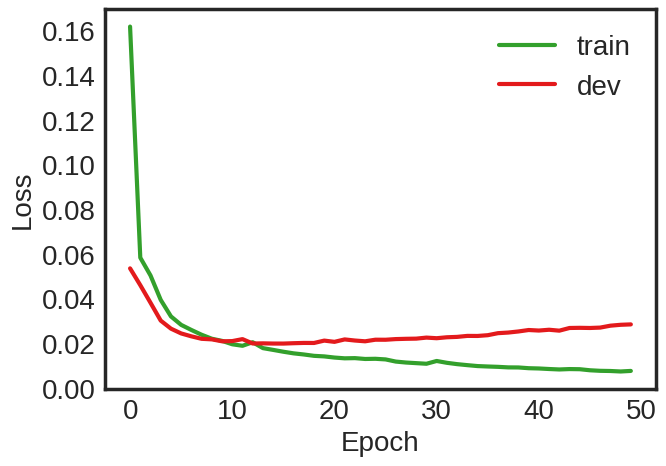
\includegraphics[height=2in]{final_test_6_loss.png}
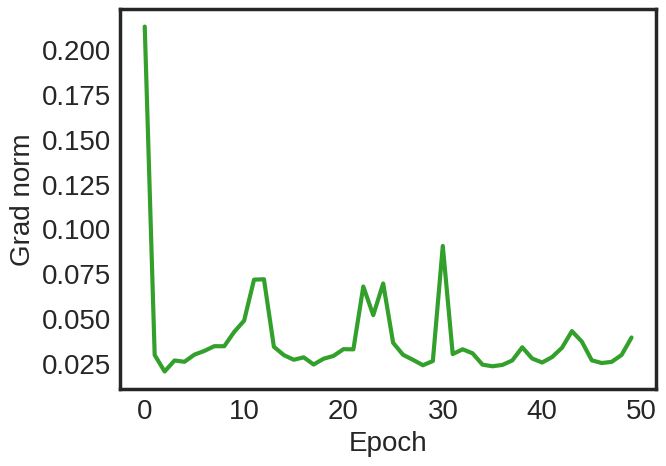
\includegraphics[height=2in]{final_test_6_grad_norm.png}
\caption{At left, a typical loss function from our training runs. The increase in the dev loss after $\sim 10$ epochs indicates overfitting, so we use early stopping to save the best model before overfitting begins. At right, a plot of the grad norm during training showing that we did not have any exploding gradient problems.}
\label{fig:loss}
\end{figure}

We also implemented gradient clipping, to ensure that our gradients didn't explode during backpropagation, but due to the LSTM architecture (see discussion in section \ref{sec:lstm}), the norm remained low enough during training that clipping was unnecessary (see right hand panel of Figure \ref{fig:loss}).

\subsection{Evaluation}

We set up a evaluation pipeline to automatically plot ROC curves and precision-recall curve for classification of each toxicity type. The pipeline also computed the ROC AUC and average precision (AP) for classification of each toxicity type, and the mean column-wise ROC AUC and mean column-wise average precision across all toxicity types. We submitted our model predictions on a test set of 153,164 comments whose true labels were withheld by Kaggle. Our online submissions returned the mean column-wise ROC AUC (the official evaluation metric in the Kaggle challenge) for our test set predictions.

\begin{table}[!ht]
\centering
\begin{tabular}{|c|c|c|c|c|}
\hline
Model & Dev $\langle$AP$\rangle$ & Dev $\langle$ROC AUC$\rangle$ & Test $\langle$ROC AUC$\rangle$ \\ \hline
Baseline & .5610 & .9669 & .9490 \\
LSTM & .5473 & .9683 & .9435 \\ 
Bidirectional LSTM & .5882 & .9747 & .9611 \\
Bidirectional LSTM + Attention & \textbf{.6695} & \textbf{.9859} & \textbf{.9778} \\
\hline
\end{tabular}
\caption{A summary table of the results from the primary models we investigated, showing the mean average precision and mean ROC AUC from the dev set, and the mean ROC AUC from the blind test set.}
\label{tab:results}
\end{table}

The results for our four primary models are shown in Table \ref{tab:results}, highlighting the substantial improvement in our multi-label classification resulting from our implementation of word attention.

\begin{figure}[ht]
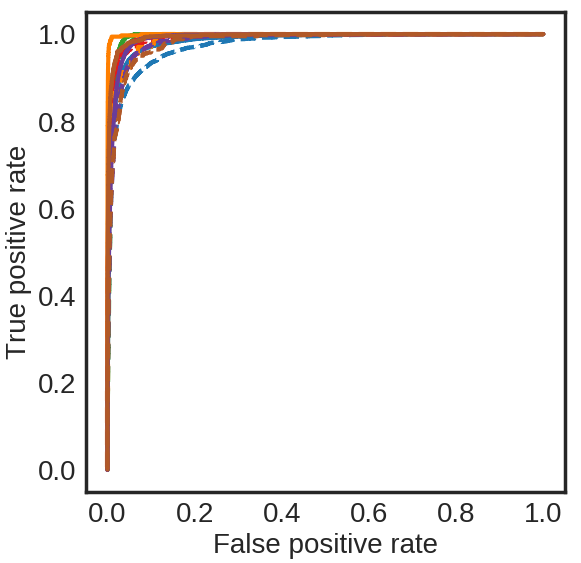
\includegraphics[height=2in]{final_test_1_big_roc.png}
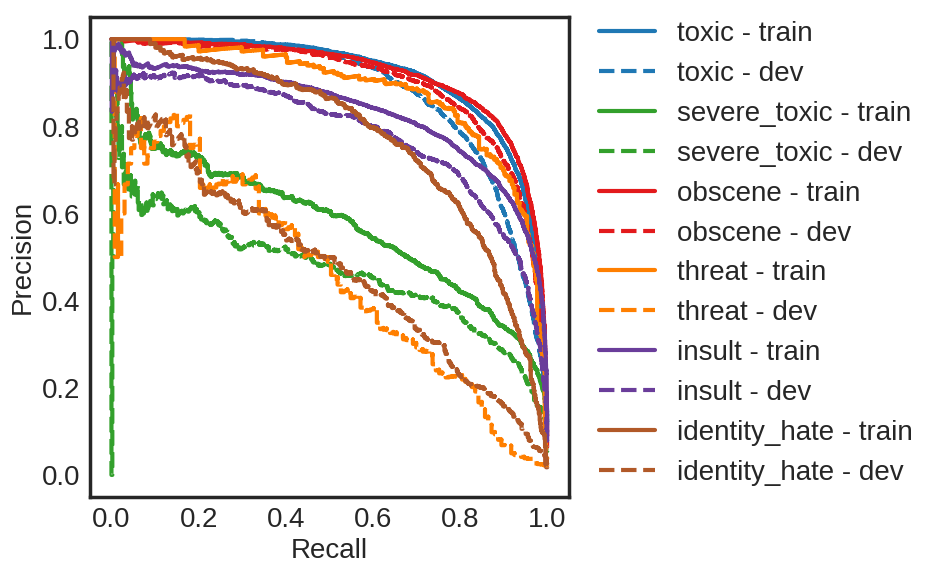
\includegraphics[height=2in]{final_test_1_big_prc.png}
\caption{The ROC and precision-recall curves for our final model.}
\label{fig:roc_final}
\end{figure}

Looking at Figure \ref{fig:roc_final}, we see that the overall performance of our final model (bidirectional LSTM + attention) is very good, with the ROC very close to the upper-left corner representing perfect classification. In the right-hand panel, we see that the classes for which we have the weakest performance are the ones for which we have the fewest training examples (\texttt{threat}, \texttt{severe\_toxic}, and \texttt{identity\_hate})

Some amount of overfitting is present, as evidenced by the dotted dev lines being displaced from the solid lines representing the performance on the training data. One way to further improve this model would be increasing the strength of the regularization beyond the dropout we have already applied.

\subsection{Qualitative Evaluation via Attention}

With its attention mechanism, our model is capable of computing the normalized attention weights ${\alpha_t}$ for every word given a sentence. For diagnostic purposes, we can visualize the attention weights of selected comments in order to qualitatively understand how the classifier classified comments the way it did. For example, here are the visualizations of the attention weights of some example true positives - in this case, comments that got successfully classified as \texttt{toxic} and \texttt{threat}:

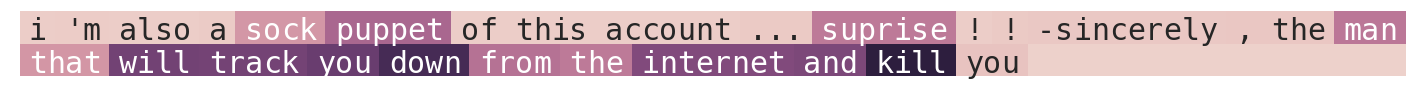
\includegraphics[width=\textwidth]{true_positive_toxic_threat_1.png}
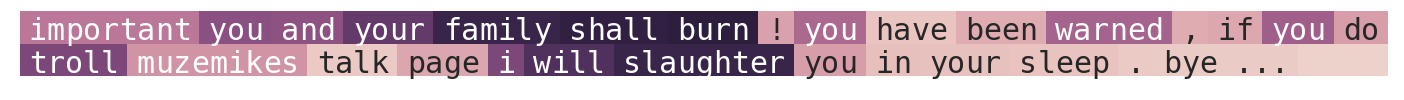
\includegraphics[width=\textwidth]{true_positive_toxic_threat_2.png}

The attention weights successfully highlight the words and phrases that sound threatening to the other users. 
 
Here is an example of a true negative:

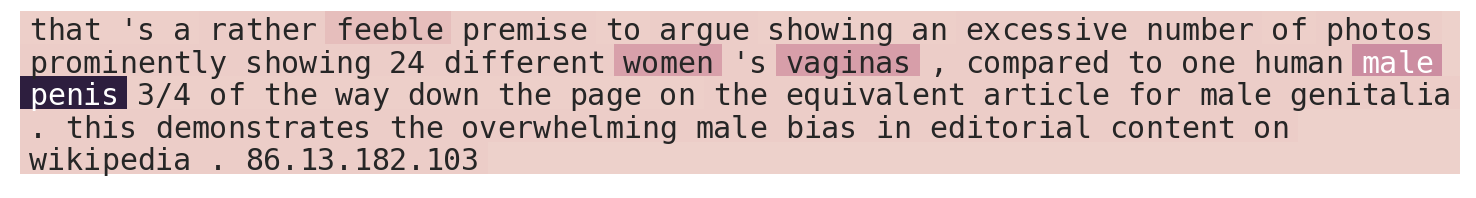
\includegraphics[width=\textwidth]{true_negative.png}

Even though the attention weights highlight some potentially vulgar words, the classifier successfully classified it as a negative. 

On the other hand, here is an example of a false positive:

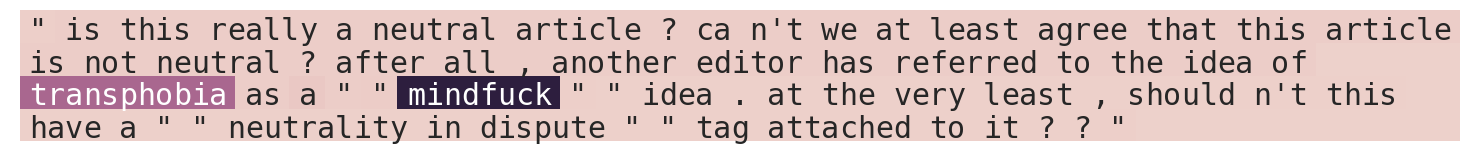
\includegraphics[width=\textwidth]{false_positive_toxic_obscene.png}

The model identifies a couple of words that could potentially be toxic, as highlighted by the attention weights, but does not pick up that the commenter is quoting someone else to make a reasonable argument, and therefore misclassifies it as \texttt{toxic} and \texttt{obscene}.

%Overall, we find qualitatively reasonable performance of both the model and the attention layer, with many 

%And finally, an examples of a false negative: 

%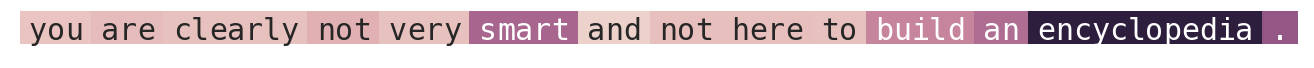
\includegraphics[width=\textwidth]{false_negative_insult.png}

%The example above was labeled as an insult but misclassified as negative. Less severe insults like this were more difficult for our model to pick up, given the general vulgarity of many of the toxic comments in the dataset. There are also 

\section{Conclusions and Future Work}

We have implemented a Tensorflow framework based on a bidirectional LSTM with an output attention layer that successfully performs multi-label classification of various subtypes of toxic online comments. Our final mean ROC AUC performance on the blind test set is .9778, which places us within .011 of the leading Kaggle entry. The addition of an attention layer to our bidirectional LSTM architecture significantly improves performance both in terms of mean column-wise ROC AUC (.9611 to .9778) and mean column-wise average precision (.5882 to .6695).

Our performance is primarily limited by the embedding of new or rarely-used obscenities to the $\langle$unk$\rangle$ token by GloVe. We tried to ameliorate this by mapping unknown composite obscenities to the embedding of the root obscenity in our preprocessing, but further such preprocessing to eliminate unknown tokens, or the use of character-level embeddings and/or convolutional methods might further improve performance, since they would be able to recognize toxic character patterns within an unknown word. In addition, stronger regularization beyond dropout might help increase the performance of our model without overfitting.

\footnotesize{
\begin{thebibliography}{9}

\bibitem{atlantic} Madrigal, A. (2017) The Basic Grossness of Humans. \textit{The Atlantic} https://www.theatlantic.com/technology/archive/2017/12/the-basic-grossness-of-humans/548330/

\bibitem{yin2009}
Yin, D., \textit{et al}. (2009) Detection of Harassment on Web 2.0. \textit{Proceedings of the Content Analysis in the WEB 2.0 (CAW2.0) Workshop at WWW2009}.

\bibitem{prevwork}
Wulczyn, E., Thain, N., \& Dixon, L. (2017) Ex Machina: Personal Attacks Seen at Scale. \textit{Proceedings of the 26th International Conference on World Wide Web}.

\bibitem{lastyear}
Chu, T., Jue, K., \& Wang, M. (2017) Comment Abuse Classification with Deep Learning. In \textit{CS224n Final Project Reports}

\bibitem{attention_paper}
Yang, Z., \textit{et al}. (2016) Hierarchical Attention Networks for Document Classification. \textit{Proceedings of NAACL-HLT 2016} 1480–1489.

\bibitem{nltk} 
Bird, S., Loper, E., \& Klein, E. (2009) \textit{Natural Language Processing with Python.} O’Reilly Media Inc. 

\bibitem{glove}
Pennington, J., Socher, R., \& Manning, C. (2014) GloVe: Global Vectors for Word Representation. \textit{Proceedings of the 2014 Conference on Empirical Methods in Natural Language Processing}.

\bibitem{gigaword} Parker, R.,  \textit{et al}. (2011) English Gigaword Fifth Edition LDC2011T07. DVD. Philadelphia: Linguistic Data Consortium.

\bibitem{relu} Nair, V. \& Hinton, G. E. (2010) Rectified linear units improve restricted boltzmann machines. \textit{Proceedings of the 27th International Conference on Machine Learning}, Omnipress, USA, 807-814.

\bibitem{xavier} Glorot, X., Bengio, Y. (2010) Understanding the difficulty of training deep feedforward neural networks. \textit{Proceedings of the Thirteenth International Conference on Artificial Intelligence and Statistics}, PMLR 9:249-256.

\bibitem{tensorflow} Abadi, M., \textit{et al}. (2015) TensorFlow: Large-scale machine learning on heterogeneous systems. Software available from tensorflow.org.

\bibitem{lstm} Hochreiter, S. \& Schmidhuber, J. (1997) Long Short-Term Memory. \textit{Neural Computation}, 9(8):1735-1780.

\bibitem{gru} Cho, K., \textit{et al}. (2014) Learning Phrase Representations using RNN Encoder-Decoder for Statistical Machine Translation, arXiv:1406.1078.

\bibitem{dropout} Srivastava, N., Hinton, G., Krizhevsky, A., Sutskever, I., \& Salakhutdinov, R. (2014) Dropout: a simple way to prevent neural networks from overfitting. \textit{J. Mach. Learn. Res.} 15 1 1929-1958.

\bibitem{attention_code}
Ivanov, I. (2018) Tensorflow implementation of attention mechanism for text classification tasks. https://github.com/ilivans/tf-rnn-attention/

\bibitem{adam} Kingma, D. P. \& Ba, J. (2014) Adam: A Method for Stochastic Optimization, arXiv:1412.6980.

\end{thebibliography}
}
\end{document}
